\newpage
\section{Funktionale Anforderungen}
Im folgenden Abschnitt betrachten wir die funktionalen Anforderungen an die Drunken-Jukebox. Dabei unterscheiden wir zwischen den beiden Akteuren Gastgeber und Gast.

\subsection{Anwendungsfälle}
\subsubsection{Gastgeber}
Für den Gastgeber haben wir drei Anwendungsfälle identifiziert. Als Gastgeber ist er für das Starten und Beenden einer Party verantwortlich, sowie für das Abspielen der Musik. Darüber hinaus verwaltet er die Songsammlung, aus der Songs für die entsprechende Party ausgewählt werden können. Die initiale Playlist wir anhand eines Algorithmus erstellt (siehe Abschnitt \ref{sec:SongSelect}).

\begin{figure}[H]
\centering
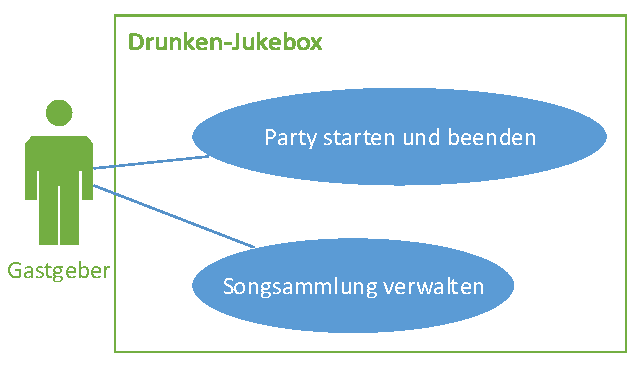
\includegraphics[width=0.75\linewidth]{Bilder/AdminUseCase}
\caption{Anwendungsfälle des Gastgebers}
\label{fig:AdminUseCase}
\end{figure}

\newpage
\subsubsection{Gast}
Die Anforderungen aus Sicht des Gastes sind etwas umfangreicher. Der Gast der Party möchte die Playlist und den aktuell abgespielten Song abrufen können. Innerhalb der Playlist möchte er die Songs bewerten und darüber hinaus seine bisherigen Bewertungen einsehen. Des Weiteren kann sein Betrunkenheitsgrad gemessen und einsehen werden.

\begin{figure}[H]
\centering
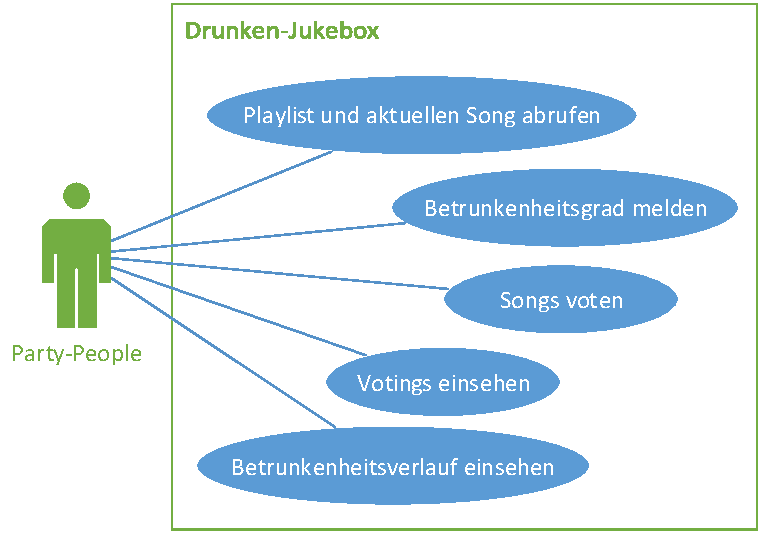
\includegraphics[width=0.95\linewidth]{Bilder/PartyPeopleUseCase}
\caption{Anwendungsfälle des Gastes}
\label{fig:PartyPeopleUseCase}
\end{figure}
